
\section{Exemplar-NBNN, an Exemplar-based Detection Model} % (fold)
\label{cha:linking}

NBNN classification and Chum's exemplar model detection \cite{chum2007exemplar} can be combined into a new detection method, because the exemplar model has more in common with the NBNN approach than most other detection methods. Exemplar models are based on image-to-class distance, like NBNN. This provides a natural way of linking both methods.

Chum \emph{et al.}\cite{chum2007exemplar} uses interest point detectors and a codebook approach for their exemplars. The descriptor space is quantized like regular codebook classification methods do, even though they take the location of the object relative to the descriptor as basis for clustering the visual words, and not the descriptors themselves.

In contrast to codebook methods however, in Exemplar-NBNN the exemplar models use image-to-class distance when testing. Like explained in Section~\ref{sub:boiman_s_nbnn}, while most codebook methods compare images to each other, in exemplar model detection the individual features are compared to the quantized exemplars. Because these exemplars have a designated class the distance of a query image to each class forms the basis for classification, and not the distance between images.

In this way, the un-quantized descriptors of NBNN can be used as exemplars. In the detection phase, using the NBNN approach, each descriptor in a query image will get a NN from a class, but also an exemplar associated with this neighbor descriptor. When the query descriptor and its NN-exemplar are combined, a hypothesis can be formed for the location of an object, in the form of a bounding box.

These hypotheses could be used as detections, using the distance of the query descriptor to the nearest class as weight. This does not totally agree however with the requirement within the NBNN approach that the classification (detection in this case) should be based on as many descriptors as possible. In this case a single detection is based on a single descriptor only. Therefore, the hypotheses should be aggregated into clusters first. Detections based on these clusters have a much larger evidence base as the cluster size gets larger. Therefore, the cluster size can be regarded as a good weight for the resulting detections.

In their implementation, Becker \emph{et al.} \cite{becker2012codebook} rank their detections in this way, breaking ties for detections of the same cluster size by comparing the mean of some relative distance measure $Q_H$ over all hypotheses that are member of the cluster. $Q_H$ is defined as follows: $Q_H=\frac{d^- - d^+}{d^+}$, where $d^+$ and $d^-$ represent the NN distance to the foreground and background class, respectively. In a multiple class setting, the background distance is the minimum over all non-class NN distances.

\subsection{Descriptor Aliasing} % (fold)
\label{sec:descriptor_aliasing}

An issue that arises using exemplar-NBNN detection is that certain descriptors may be very similar to not one, but multiple neighbors. These neighbors might refer to totally different exemplars, generating a variety of hypotheses. This effect can be called descriptor aliasing, and is shown in Figure~\ref{fig:aliasing}.


\begin{figure}[hbt]
    \centering
    \begin{subfigure}[b]{0.45\textwidth}
        \centering
        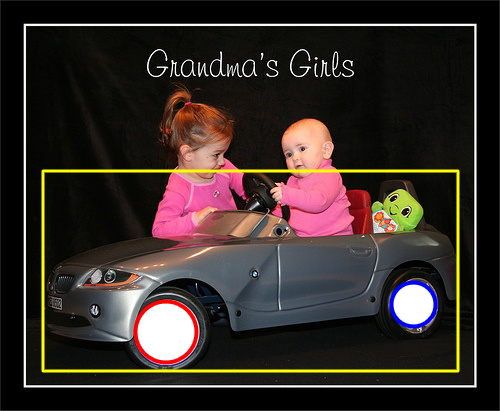
\includegraphics[width=\textwidth]{aliasing}
        \caption{Training image}
        \label{fig:aliastrainim}
    \end{subfigure}
    ~
    \begin{subfigure}[b]{0.45\textwidth}
        \centering
        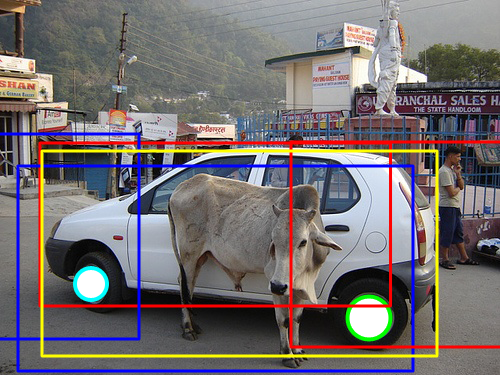
\includegraphics[width=\textwidth]{aliasing2}
        \caption{Test image}
        \label{fig:aliastestim}
    \end{subfigure}
    \caption{During training (a), each descriptor gets an exemplar from ground truth, in this case the descriptors for the car's wheels. During detection (b), each descriptor found (again car wheels), gets hypotheses based on its neighbors for each class. Here, the wheel's two neighbors are those of (a), and their hypotheses are given in blue and red respectively (ground truth is given in yellow). When only one neighbor is taken into account, there is a risk of not favoring the two more or less correct bounding boxes because of repetition of descriptors in the training images.}
    \label{fig:aliasing}
\end{figure}

\todo{Insert a third image after clustering, with cluster sizes, perhaps exchange it for a real result?}

This problem can be avoided by taking more than one neighbor into account, which translates to setting $k>1$ in the $k$NN phase of exemplar-NBNN. This would mean that all $n\leq k$ neighbors that are closer to the foreground than the nearest background descriptor will be used to make detection hypotheses. This is not only an argument for introducing LNBNN detection, but also in general, for taking into account more neighbors in regular NBNN detection. This phenomenon explains some of the results obtained in the experiments.

% section descriptor_aliasing (end)

% chapter linking (end)
